%!TEX root = ../thesis.tex
\chapter{Introduction}
\label{chap:introduction}

The majority of the stars and brown dwarfs forms in stellar clusters. \citet{2000AJ....120.3139C} reports that $50-70\%$ of very young ($\leq10$ millions of years, in the following Myr) and $25-70\%$ of the young ($\leq100$ Myr) stellar populations are formed in clusters. \citet{2003AJ....126.1916P} and \citet{2003ARA&A..41...57L} find that among 80\% to 90\% of the stars are formed in clusters with more than 100 members. Furthermore, as indicated by the former authors, these clusters ($\geq$100 members) represent 22\% of the regions where stars form. The remaining of the star forming regions are small associations, with 5 to 30 members, where only up to 10\% of the stars are formed. However, only less than 7\% of the clusters ($\geq 100$ members) survives as gravitationally bounded clusters when reaching an age of a few hundred Myr \citep{2003ARA&A..41...57L}. The remaining (93\%) of the star forming regions will become unbounded and their stars will freely populate the galaxy. Thus, to understand the general rules that govern how the majority of stars forms, as well as the properties of the stars that populate our galaxy, it is crucial to fully decode the formation and early evolution of stellar clusters. 

Astrophysicists, like archeologists and palaeontologists, can not willingly reproduce the vast majority of their studied phenomena. Although some experiments can be performed in specific situations (e.g. the chemical and physical  properties of dust and gas) astrophysics remains an observational science. For this reason, to test the validity of their hypotheses, astrophysicists relay on statistical studies carried out over carefully designed observations. In particular, the understanding of the star formation process requires carefully designed observations of  stellar clusters whose ages cover the early stages of cluster evolution.

The objective of this work is the construction, test and validation of an statistical tool, an intelligent system specifically, that given the data of carefully designed observations of an stellar cluster, recovers the statistical distributions of its population. In particular, it delivers the luminosity distribution, which can be transformed into the mass distribution, given an evolutionary model and cluster age. The mass distribution is the fundamental product of the star formation process. It contains the fingerprints of the early phases of star formation and subsequent cluster evolution.

An homogeneous and precise mass distribution inventory for clusters of diverse ages and forming environments will allow the astrophysical community to test the current theories of the star formation process. In particular, it will allow to solve the questions about universality of the initial mass distribution (function) and the role play by the physical properties of the cluster environment.    

The remaining of this Chapter is structured as follows. In Section \ref{sect:IMD}, I describe the importance of the initial mass distribution and some of its current models. In Section \ref{sect:numerical_simulations}, I report the current developments of the numerical simulations of cluster formation. In Section \ref{sect:DANCeproject}, I describe the project DANCe and its carefully designed observations of stellar clusters; the ones used in this work. In Section \ref{sect:current_methodologies}, I comment on the current methodologies for the analysis of star clusters and associations. Finally in Section \ref{sect:newtool}, I briefly describe the methodology adopted for this new statistical tool, and the advantages over the previous works. 

\section{The initial distribution of masses}
\label{sect:IMD}

The measuring and understanding of the initial mass distribution is a central topic in the study of star formation. It is also essential in other areas of astrophysics, from planetary formation, where it appears that the mass of the host star plays an important role in the formation of the planetary system \cite[see for example][]{2015ApJ...814..130M}, to galactic evolution \citep{1998ASPC..142....1K} and cosmology \cite[see for example][]{2012MNRAS.423.3601N}. 

The theories that predict the origin of the initial mass distribution can be categorised into deterministic and stochastic \citep{Offner2014}. The former postulate that stellar masses are deterministically inherited from the initial core masses via accretion from the gas reservoir of the parent molecular cloud. Thus, the initial mass distribution can be directly mapped from the distribution of initial core masses, and the understanding of the former reduces to that of the latter. On the other hand, stochastic models postulate that the stellar masses are independent of the initial core masses. Among these models, there are those proposing that stellar masses are determined by dynamical interactions and contest for gas. For more details see \citet{Offner2014} and references therein. 

  The observational studies of the initial mass distribution are conditioned on the ages of the stellar populations under analysis, and relay deeply on the assumed processes that link the observed present-day mass distributions (PDMDs) to the initial one. While the resulting models for the initial mass distribution are always analytical functions of the mass, the observed PDMDs are commonly expressed with points, histograms or kernel density estimations\footnote{KDEs are non-parametric ways to estimate a probability density function by means of an independently and identically distributed sample drawn from it.} (KDEs). In the following and for the sake of simplicity, I refer to the analytical functions of the initial mass distribution as the Initial Mass Functions (IMFs). 

The most common IMFs are the log-normal functions of Chabrier \citep{Chabrier2003,Chabrier2005}, the power-law functions of Salpeter \citep{Salpeter1955}, Miller and Scalo \citep{Miller1979}, and Kroupa \citep{Kroupa2001,Kroupa2002,Kroupa2013,Thies2007,Thies2008}. Other functional forms include the truncated exponential \citep{deMarchi2001} and the Pareto-Levy distribution \citep{Cartwright2012}. In behalve of simplicity, I will only explain the most classical ones of Chabrier and Kroupa.


- The initial mass function of \citet{Chabrier2003,Chabrier2005,Thies2007}
\citet{Chabrier2005} found this function by fitting a log-normal function to the visual luminosity distribution of the closest $8$ pc field objects.

\section{Numerical simulations of the early stages of star formation}
\label{sect:numerical_simulations}

In the first decade of this century, numerical simulations of star forming regions have proved to be of paramount importance in the decoding the very early stages of the star formation process \citep{2003MNRAS.339..577B,2005A&A...435..611J,2009MNRAS.392..590B,2009MNRAS.392.1363B,2009MNRAS.397..232B}. For example, \citet{2003MNRAS.339..577B} using smooth particle hydrodynamics were able to simulate the collapse and fragmentation of a large-scale ($50 M_{\odot}$ within 0.375 pc radius) turbulent molecular cloud to from a stellar cluster. During the very first 0.1 Myr of the star formation process, the time covered by the simulation, they were able to simultaneously form discs and binary stars. The cloud formed roughly equal numbers of stars and brown dwarfs (23 and 27, respectively) resulting in a mass distribution with a flat slope in the range $0.01-0.5 M_{\odot}$; see Fig. \ref{fig:IMFBate2003}. \citet{Offner2014} provides a review of the stellar initial mass distribution (function), and of the physical effects included in numerical simulations (radiative feedback, competitive accretion, dynamical interactions, magnetic fields) particularly. 

In recent years, the works of \citet{2015ApJ...815...27K} and \citet{2015MNRAS.452..566B}, using the cold collapse paradigm (neglecting magnetic fields, radiative transfer and feedback), were able to probe that the main source driving the star formation process is gravity. Their simulations were typically run until 0.85 Myr in a box of 3 pc of side, and with masses in the few thousands of $M_{\odot}$. In particular, the mass distribution obtained by \citet{2015ApJ...815...27K} reproduces reasonably well the current models of the initial mass distribution (see Fig. \ref{fig:IMFKuznetsova}).

% Remaining issues

Numerical simulations have proven to be of great use in the understanding of the star formation process in stellar cluster, in the very early phases ( $\leq$1 Myr) of their evolution particularly.  Despite the fact that many of these simulations are in agreement with the observed mass distributions, currently they do not incorporate all astrophysical effects, resolve close binaries or produce enough stellar objects \citep{Offner2014}. 

- The problematic of constraints in dynamical theories.

% Why are these issues important?
\begin{figure}[htbp]
\begin{center}
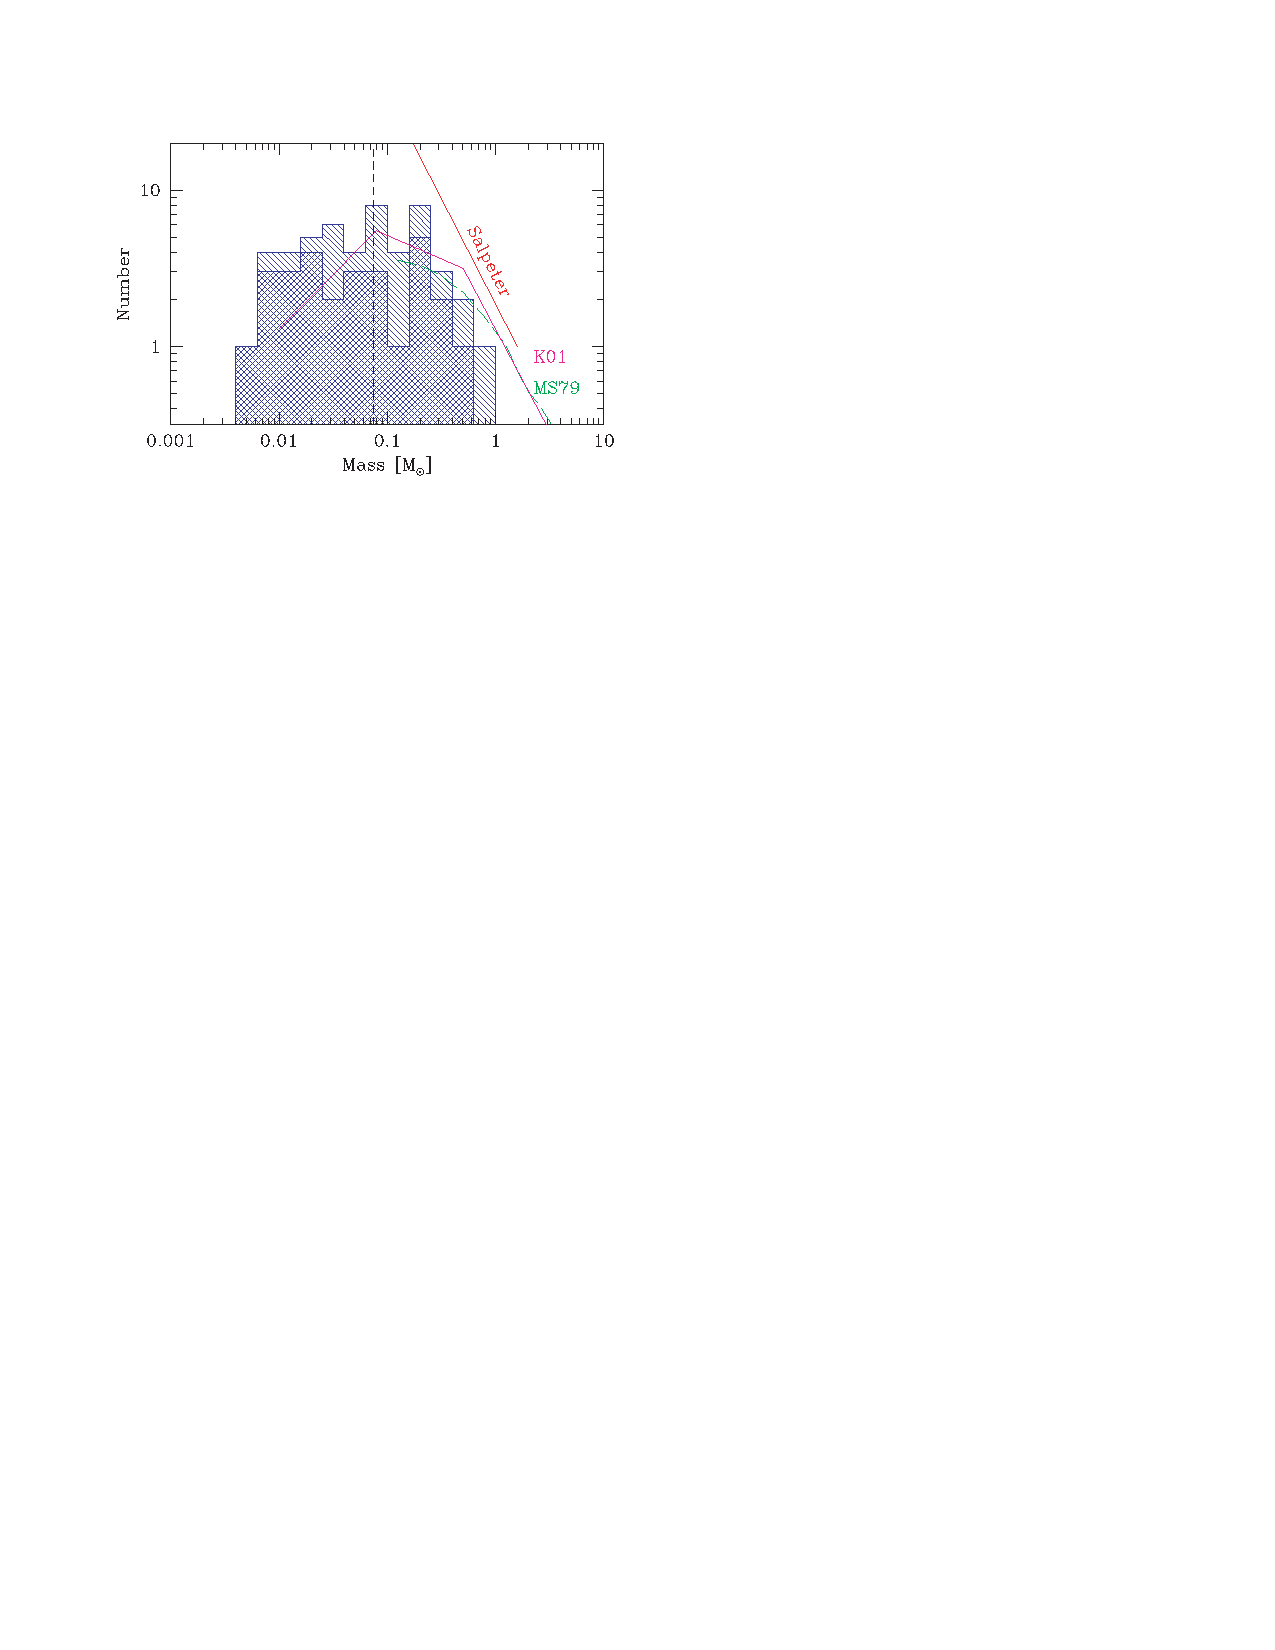
\includegraphics[width=0.8\textwidth]{background/Figures/F10_Bate2003.pdf}
\caption{Mass distribution resulting from the numerical simulation of \citet{2003MNRAS.339..577B}. The lines show the mass distributions of \citet{Salpeter1955}, \citet{Miller1979} and \citet{Kroupa2001}. Reproduced from Figure 10 of \citet{2003MNRAS.339..577B}}
\label{fig:IMFBate2003}
\end{center}
\end{figure}

\begin{figure}[htbp]
\begin{center}
\includegraphics[width=0.8\textwidth]{background/Figures/F11_Kuznetsova.pdf}
\caption{Mass distribution resulting from the numerical simulation of \citet{2015ApJ...815...27K}. The High (solid line) and Low (dashed line) resolution simulations reach $0.05\, M_{\odot}$ and $0.15\, M_{\odot}$, respectively. Also shown the mass function of \citet{Chabrier2005} (red dashed line). Reproduced from Figure 11 of \citet{2015ApJ...815...27K}}
\label{fig:IMFKuznetsova}
\end{center}
\end{figure}

\section{The DANCe project}
\label{sect:DANCeproject}
It must be clear which is the objective

Description of the Nearby open clusters and their properties.

- List of open clusters in the DANce project.

- the importance of the pleiades, why we restrict to it.

It must be clear what are the limitations, the boundaries in which the objective will be searched

\section{Current methodologies}
\label{sect:current_methodologies}
Description of the current methodologies used to address the question mentioned previously.

- The works of Sarro, Krone-Martins, Malo, Gagne etc. LAcweing

-The advantages and caveats of the previous methodologies. 

-It must be clear the necessity of a new perspective

\section{The new tool}
\label{sect:newtool}

The proposal we made. The use of Bayesian Hierarchical Models. Benefits and issues of BHM.

Description of the advantages of BHM.

-> It must be clear that BHM are the best choice.

Description of the practical issues needed to be solved in order to use BHM.

MCMC techniques and  PSO.

-> It must be clear that MCMC methods are the best option.

Brief descriptions of our results and how they impact our current knowledge.

-> It must be clear that we attained the objective: The pleiades velocity, spatial and mass distributions.
 



